\section{Co-compression}
\label{sec:co_comp}

In sections \ref{sec:n_gram} and \ref{sec:machine_learning}, we explored leveraging an understanding of a text's regularities for compression. This section explores the opposite idea, namely using an existing compression algorithm as a black box to understand regularities in text.

One point of commonality between compression and comprehension is the need for parsimony. This is expressed by Occam's razor, which states that "entities must not be multiplied beyond necessity" and commonly understood to mean that "the simplest explanation is usually the best one".

Compression algorithms, for example the family of Lempel-Ziv algorithms, in fact operate by eliminating the multiplication of entities through the creation of a \emph{codebook}, a mapping between often-repeated bits of data and what is essentially an abbreviation for each. If the relationship between compression and comprehension holds, we should expect to be able to use an existing compression algorithm like LZMA to get a rudimentary understanding of text.

\textcite{Jiang2023} showed that it's possible to use gzip for text classification, based on

\begin{displayquote}
"the intuitions that
\begin{enumerate}
\item compressors are good at capturing regularity; 
\item objects from the same category share more regularity than those from different categories"
\end{enumerate}
\end{displayquote}

To illustrate this using the same dataset of 97 Gutenberg texts, I use the following scoring methods to estimate the similarity of a pair of texts:

\[add(y|x) = \frac{C(xy) - C(x)}{C(y)}\]

where \(C(t)\) is the compressed length of \(t\) expressed in bytes, and \(xy\) is the concatenation of the texts \(x\) and \(y\). The function \(add(y|x)\) is then a measure of the additional information given by \(y\) when \(x\) is taken as a known basis.

To give an intuition for why the measure is defined in this way, it's helpful to use an example. Suppose that $x$ is the text of the complete works of Shakespeare and that $y$ is the text of Romeo and Juliet. Since $x$ contains $y$ as a substring, we should expect that a good compression algorithm would compress the concatenation $xy$ in little more space than is required for just $x$, as the entire text of $y$ can be signified with a single symbol in the codebook, compressed once, and referred to twice.

Because of this, we should expect the value of $add(y|x)$ in this case to be close to 0, corresponding to the fact that $y$ does not really add information to $x$. Conversely, since the complete works of Shakespeare contain a lot of information not contained in just Romeo and Juliet, we should expect $add(x|y)$ to be close to 1, indicating that our compression algorithm's knowledge of the text of Romeo and Juliet only makes a small dent in the number of additional bits it needs to represent the works of Shakespeare.

The measure used above contrasts with Normalized Compression Distance (NCD) as used by \textcite{li2004similarity} , in that it is directional, i.e. that \(add(x|y)\) is not necessarily equal to \(add(y|x)\).

We may also define a more intuitive similarity score as follows

\[similarity(y|x) = 1 - add(y|x) = \frac{C(x) + C(y) - C(xy)}{C(y)}\]

This score giving a measure of the similarity of \(y\) to \(x\). In this case, $similarity(a|b)=1$ would indicate that $a$ is fully described by $b$ (as it contains no additional information), and $similarity(a|b)=0$ indicates that $a$ is unlike anything seen in $b$. Again, note that \(similarity(y|x)\) is not necessarily equal to \(similarity(x|y)\).

\begin{figure}[t]
\centering
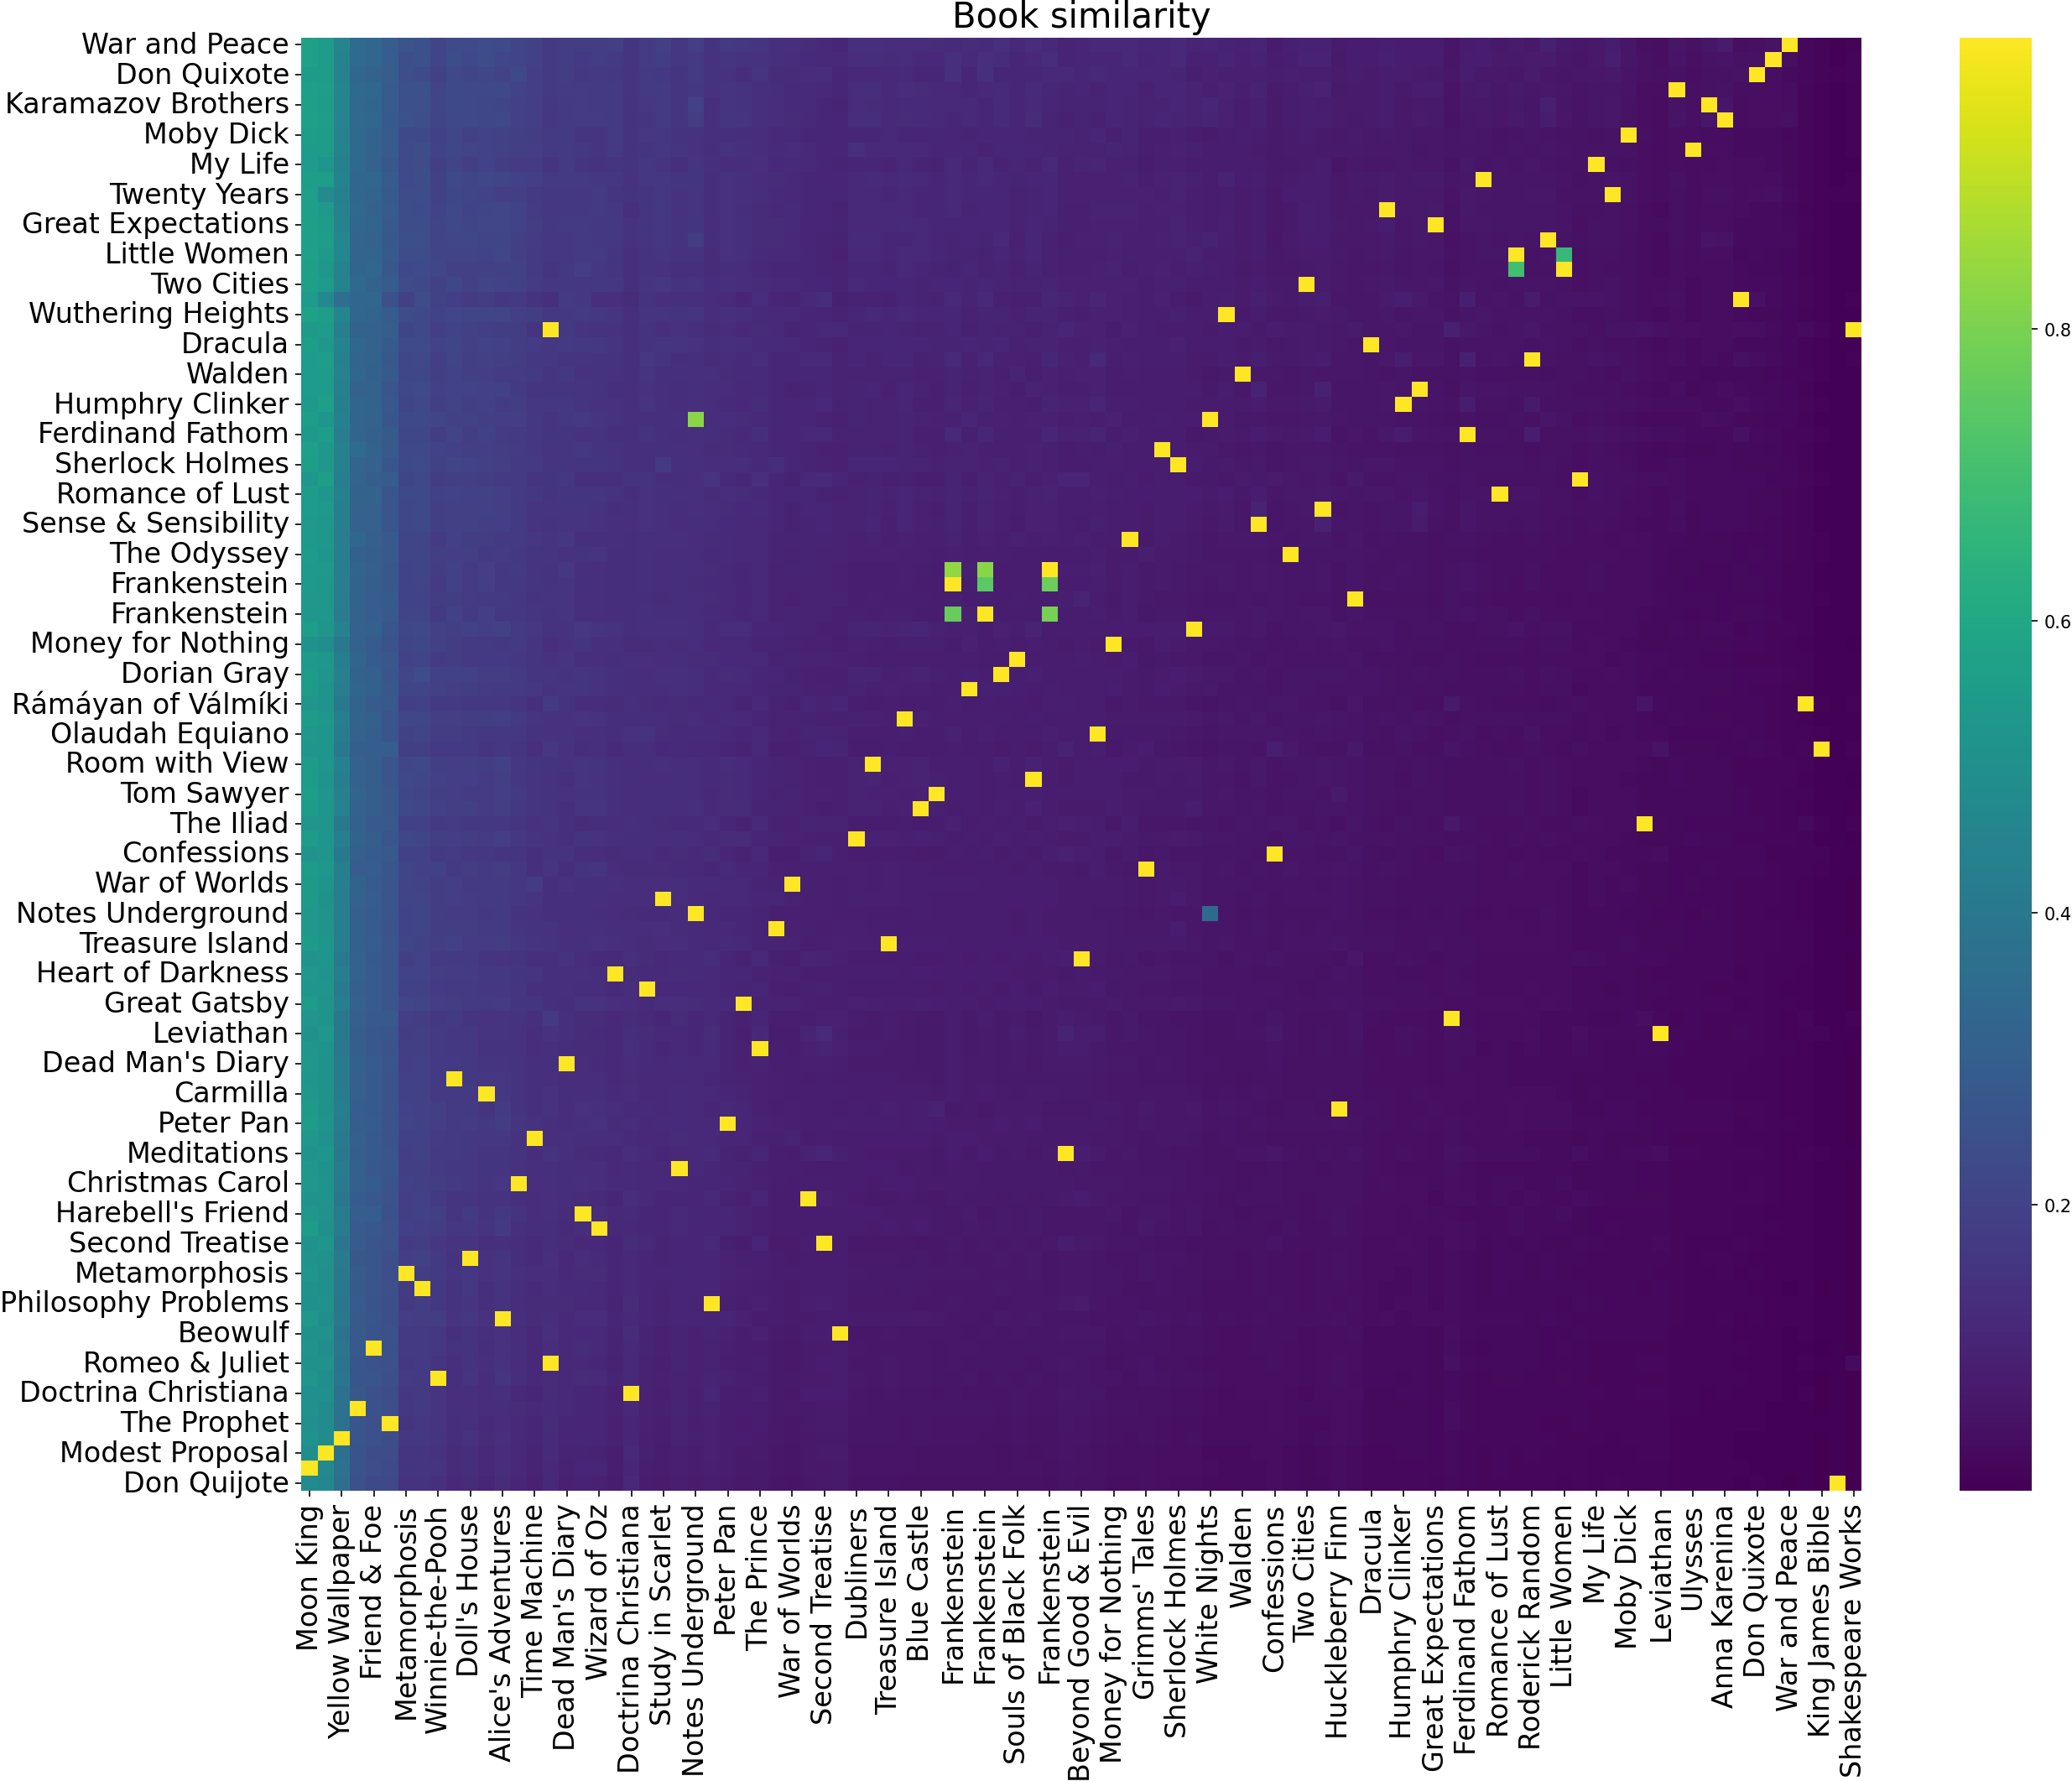
\includegraphics[width=\textwidth]{img/fig_co-compression_median.png}
\caption{Similarity scores for pairs of texts. The texts on the vertical axis are ordered most-predictive-first, and those on the horizontal axis are ordered most-predictable-first.}
\label{fig:heatmap_ppsort}
\end{figure}

\begin{figure}[t]
\centering
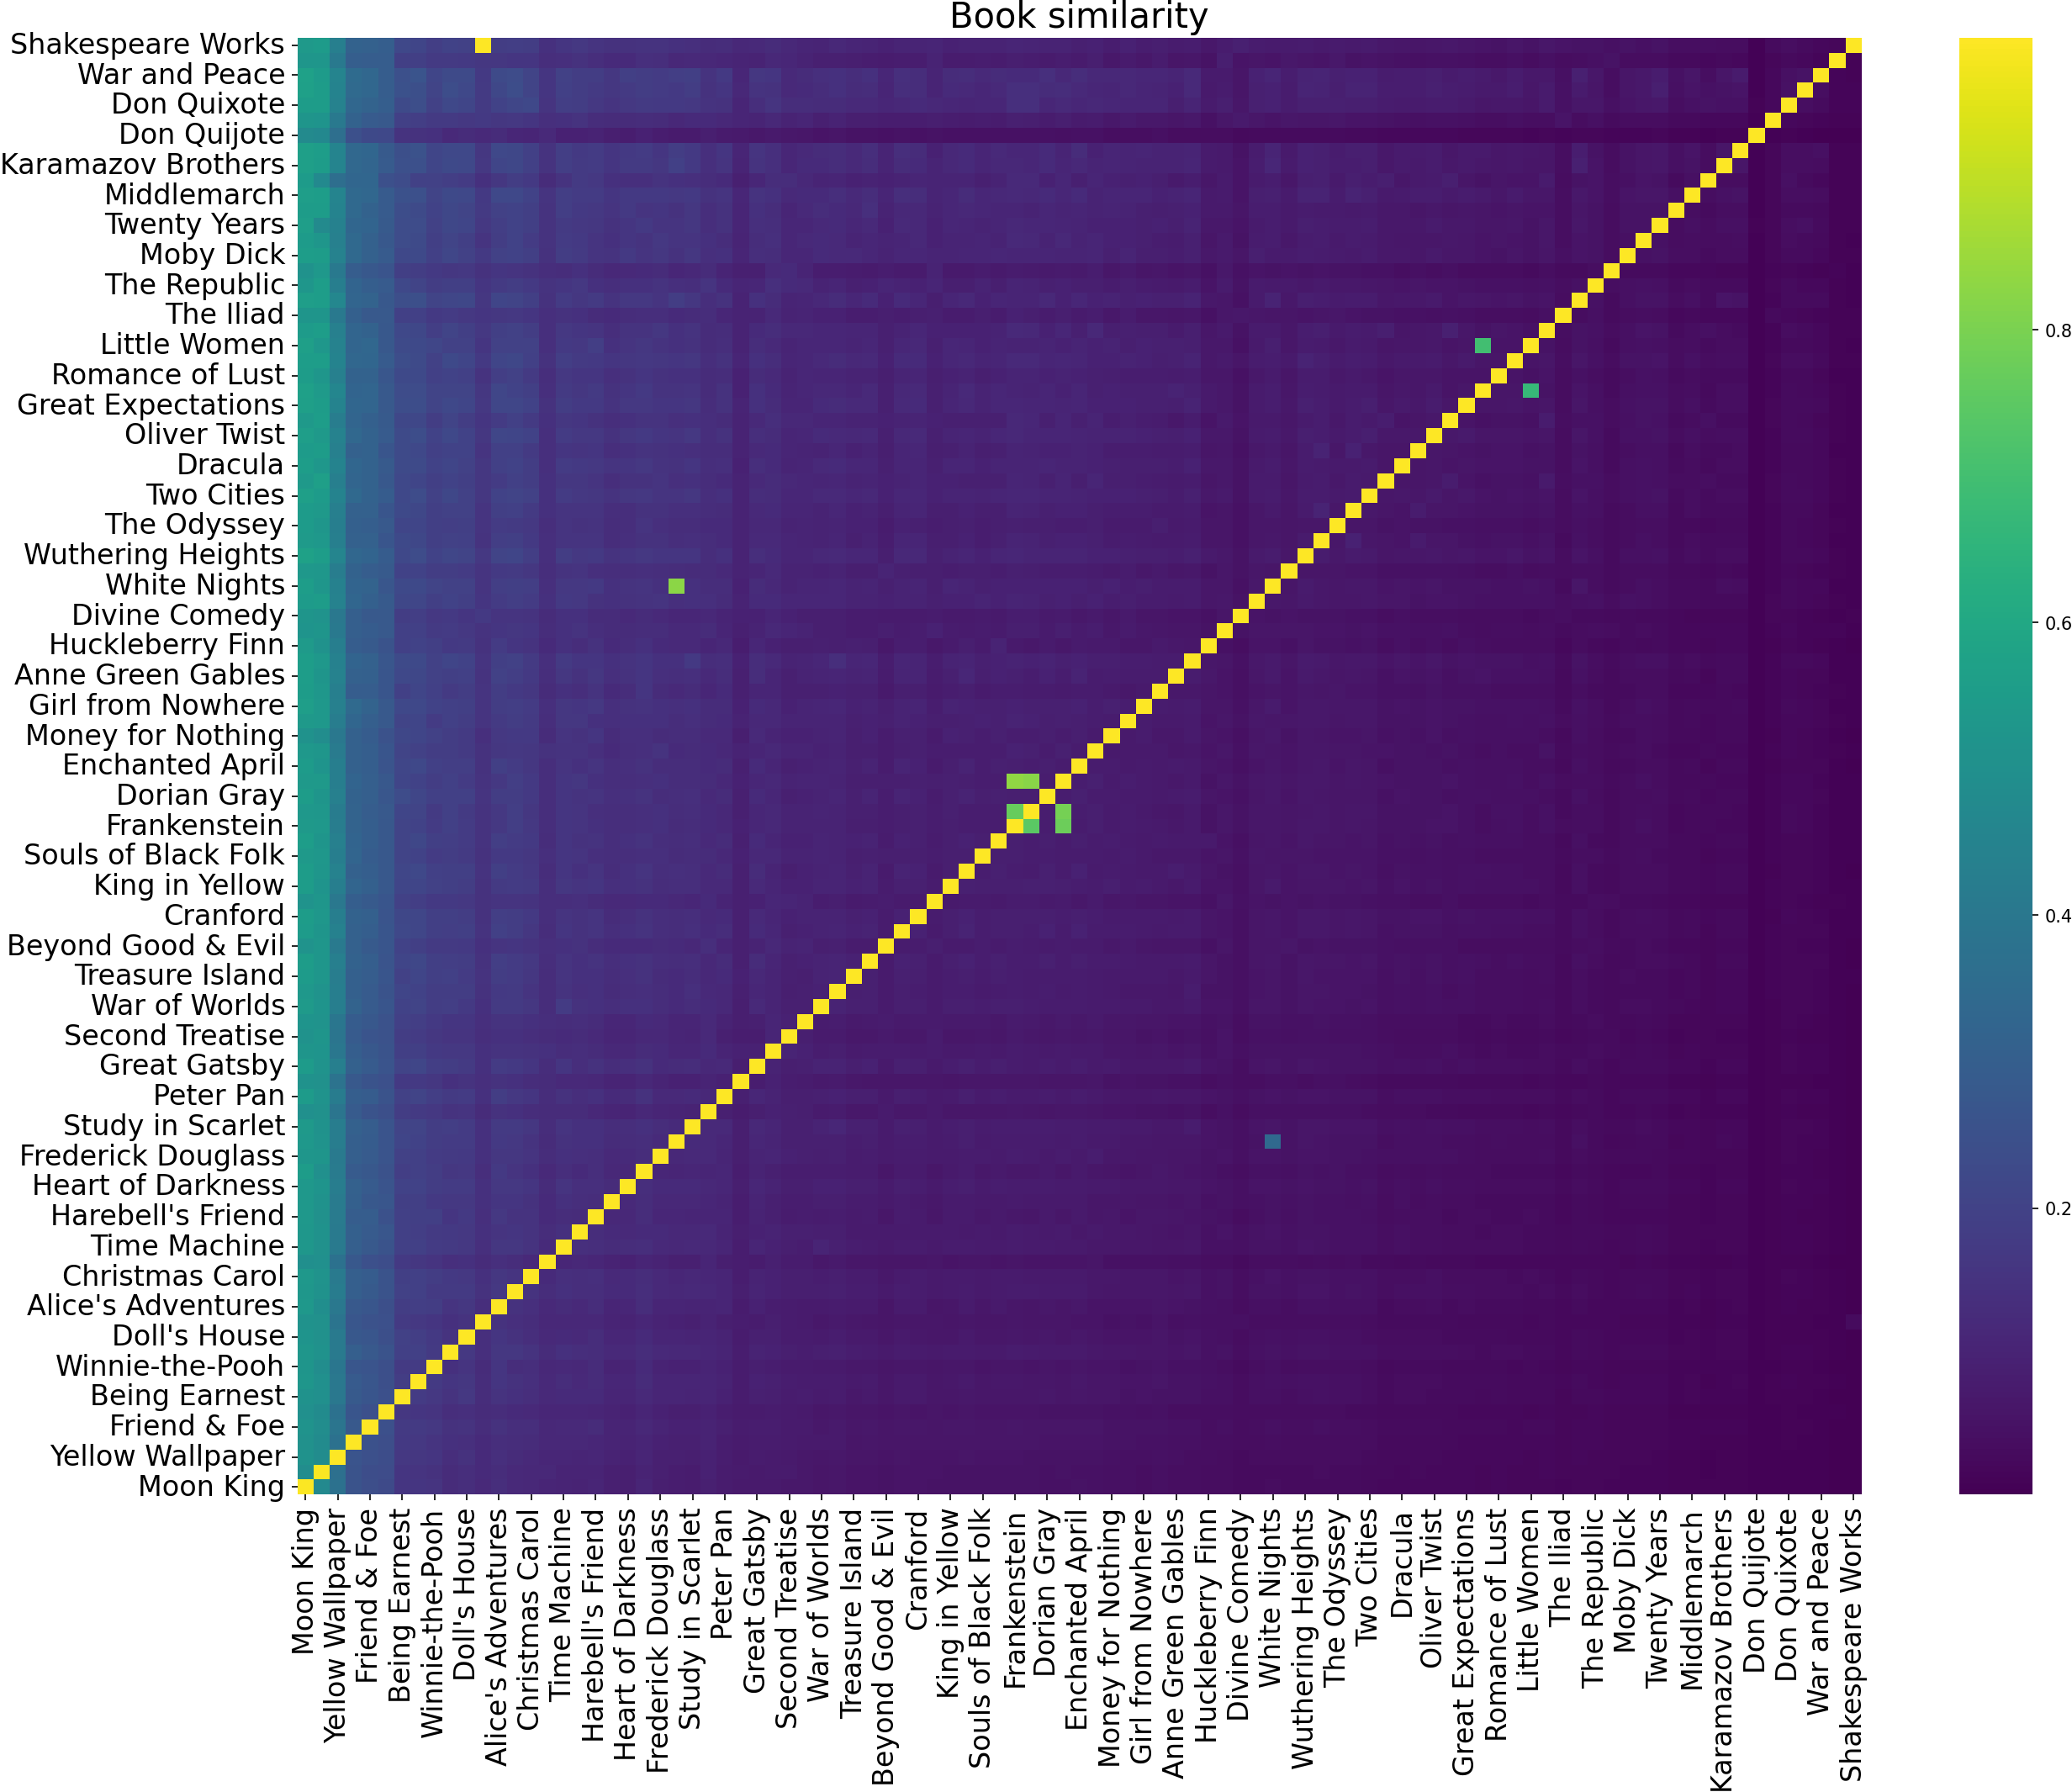
\includegraphics[width=\textwidth]{img/fig_co-compression_file_size.png}
\caption{Similarity scores for pairs of texts. The texts on both axes are sorted by file size.}
\label{fig:heatmap_fsort}
\end{figure}

This similarity score is plotted for pairs of texts in figures \ref{fig:heatmap_ppsort} and \ref{fig:heatmap_fsort}, each plot giving \(x\) on the horizontal axis and \(y\) on the vertical axis, the color of the cell representing \(similarity(x|y)\). In figure \ref{fig:heatmap_ppsort}, the texts on the vertical axis are sorted by how predictive they are on average, and the texts on the horizontal axis are sorted by how predictable they are. In figure \ref{fig:heatmap_fsort}, the same texts are instead sorted by file size on both axes.

The figures were produced the  \texttt{\href{https://github.com/Guy29/FYP/blob/main/Code/co_compression/stats.py}{co\_compression/stats.py}} script in the repository for this project. Creating the figures involved experimenting with each of 4 compression algorithm libraries (\texttt{zlib}, \texttt{lzma}, \texttt{gzip}, and \texttt{bz2}) to find the most suitable for co-compression. Since one of the functions that \texttt{stats.py} performs is to co-compress all possible pairings of texts from a set of 97, the results are serialized and saved regularly to avoid need for recalculation. The script uses the \texttt{seaborn} and \texttt{matplotlib} python libraries for generating the figures, and \texttt{pandas} is used to process and tabulate the data.

The following observations can be made based on figures \ref{fig:heatmap_ppsort} and \ref{fig:heatmap_fsort}:
\begin{itemize}
  \item In general, larger texts are more predictive.
  \item In general, smaller texts are more predictable.
  \item There are a few very bright dots which do not lie along the diagonal in \ref{fig:heatmap_fsort}. These appear because the dataset includes three versions of Frankenstein which have a high similarity score with each other, as well as the texts for Romeo and Juliet, and the Complete Works of Shakespeare. For this last pair, the latter strongly predicts the former but the former only weakly predicts the latter.
  \item There is a strong horizontal dark line in both graphs, which represents a text that is unpredictable regardless of what other text it is paired with. On inspection, this turns out to be Don Quijote, which is in fact unlike the other texts because it is in Spanish, whereas most other texts are in English.
  \item As can be seen in \ref{fig:heatmap_ppsort}, when texts are sorted most-predictive-first on the $y$-axis and most-predictable-first on the $x$-axis, texts generally lie along the diagonal. This indicates that, within a set of texts, there is a trade-off between how predictive a text is and how predictable it is. At least part of this effect has to do with file size, as larger texts tend to contain a larger set of the possible words and expressions of a language.
  \item There is a visible pattern of strong vertical and horizontal lines in \ref{fig:heatmap_fsort} (i.e. there is a low level of noise), indicating that texts tend to be "generally predictive" or "generally predictable" within a given collection.
\end{itemize}

\subsection{Practical application}
\label{subsec:co_comp_practical}

As can be seen in the previous figures, it is always the case for any two pairs of texts $x$ and $y$ that "the whole is less than the sum of its parts", i.e. that $C(xy) < C(x) + C(y)$. This opens up the question of whether it is possible to obtain a better compression of $y$ by encoding only that information which it adds to $x$. If this is possible, we should expect that this information should be of the size $C(xy) - C(x)$ which, by the previous equation, is necessarily less than $C(y)$.

Intuitively, this means that if two parties - Carol and Dave - each have a copy of the works of Shakespeare, and Carol wants to send over Romeo and Juliet, she can simply encode it by giving the range of pages on which it appears in their shared reference text, a much shorter representation than sending the actual text of Romeo and Juliet.

Is this possible to implement in practice? The fact that Lempel-Ziv algorithms work by going through the data in one pass and creating a codebook as they go indicates that $D(xy)$ should contain $D(x)$ as a prefix, where $D(t)$ stands for the compression of $t$. This is, in fact, more or less the case with LZMA, and I was able to create a simple tool that implements this idea, available at \texttt{\href{https://github.com/Guy29/FYP/blob/main/Code/libraries/co_compressor.py}{libraries/co\_compressor.py}} .

The \texttt{CoCompressor} class I implement is instantiated with two arguments: a reference text $r$ and a compression algorithm. Its \texttt{compress} method takes a text $t$ to compress and outputs $D(rt)$ with the prefix $D(r)$ removed, and its \texttt{decompress} method takes a text compressed in this way, prefixes it with $D(r)$ and decompresses it, reversing the process.

Co-compressors instantiated in this way differ in their power depending on the choice of reference text. See figure \ref{fig:cocomp_comparison} below for a comparison of the performance of co-compressors trained on different reference texts.

\begin{figure}[h]
\centering
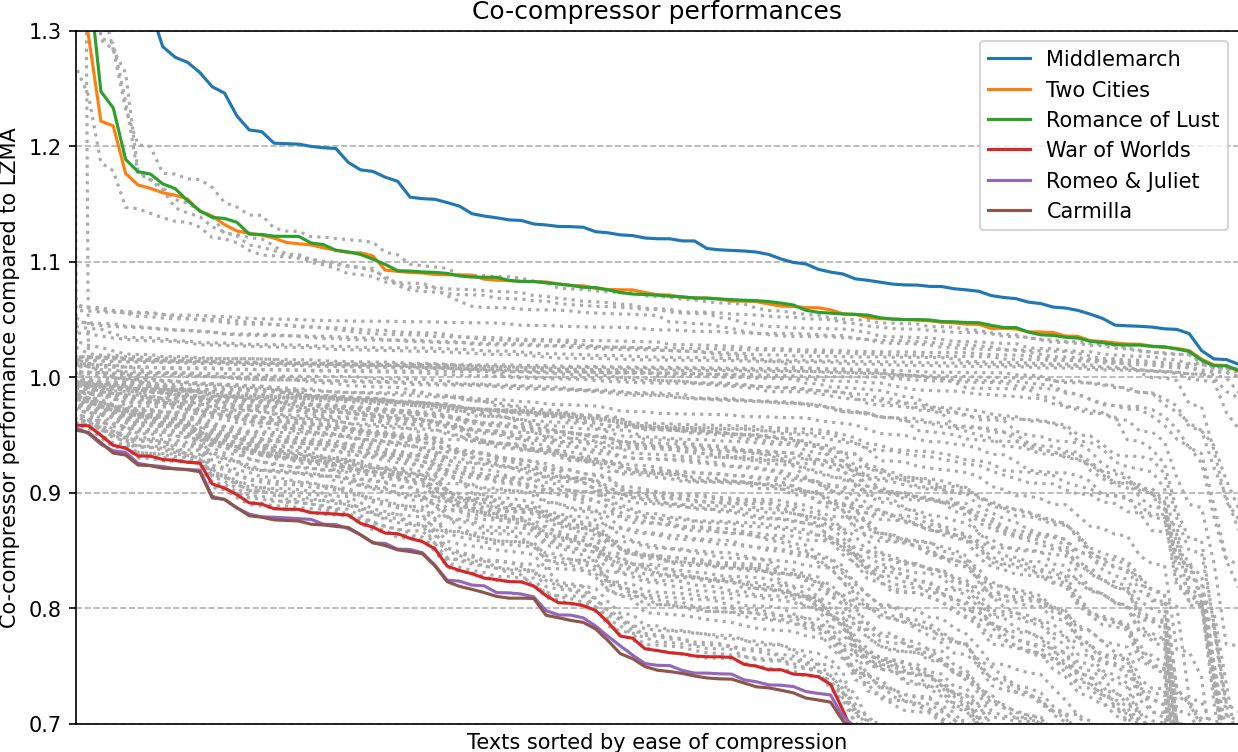
\includegraphics[width=\textwidth]{img/fig_cocomp_performance.png}
\caption{The performance of instances of the \texttt{CoCompressor} class trained on 97 different texts. Each line represents a \texttt{CoCompressor}. The value on the vertical axis is the Relative Compression Ratio (RCR), calculated as the size of the encoding produced by naive LZMA divided by that produced by the \texttt{CoCompressor}, while the horizontal axis goes through possible inputs for comrpession.}
\label{fig:cocomp_comparison}
\end{figure}

There are a few remarkable things about this figure:

\begin{itemize}
    \item Each co-compressor shows a tan- or sigmoid-like curve, performing exceptionally well on texts which are very similar to it (left side of the plot) and steeply dropping down in performance for sufficiently different texts.
    \item There is very little criss-crossing between the lines in this plot. That is, for any pair of co-compressors, one will usually outperform the other \emph{on every input} in the dataset. Why there should be a strict hierarchy of this sort is not clear, as one might expect that a specific co-compressor would be specialized for texts which are similar to it but not for others.
    \item The best performing co-compressor in this dataset is the one trained on Middlemarch (performing 12\% better than naive LZMA in the median case), followed by A Tale of Two Cities (7.3\%) and The Romance of Lust (7.2\%).
\end{itemize}

It is tempting to explain away the unusual performance of the Middlemarch co-compressor (henceforth $CC_{MM}$) as an artifact of the chosen dataset, that it might be situated (historically or otherwise) "in the middle" of the dataset, sharing some features with both preceding and following literary works.

One strong piece of evidence against this is that, as noted above, the performance of co-compressors is strictly hierarchical, and this effect extends all the way to the left of the plot where the co-compressor is fed the text it performs best on (that is, its own text) as its input. Examining this, we notice that

$$RCR_{MM}(MM) > RCR_t(t) \qquad \forall t \in G$$

where $RCR_a(b)$ is a measure of the performance of the co-compressor trained on text $a$ when fed input $b$ (as defined in figure \ref{fig:cocomp_comparison}), and $G$ is the Project Gutenberg dataset. That is, $CC_{MM}$ is not only the most performant co-compressor on all the texts in the dataset, it is also the co-compressor that performs best on its own reference text.

This observation gives a simple way to find other good reference texts for co-compressors: one simply calculates $RCR_t(t)$ for each candidate and finds values of $t$ that yield the highest performance.

I implement this method on a much larger dataset of 92600 texts downloaded from Project Gutenberg, this time only using \texttt{CoCompressor} objects trained on a text to compress the same text, and measure the relative compression ratio (RCR) for each text, where

$$RCR_a(b) = \frac{length(LZMA(b))}{length(CC_a(b))}$$

that is, the performance of the co-compressor relative to naive LZMA.

\begin{figure}[h]
\centering
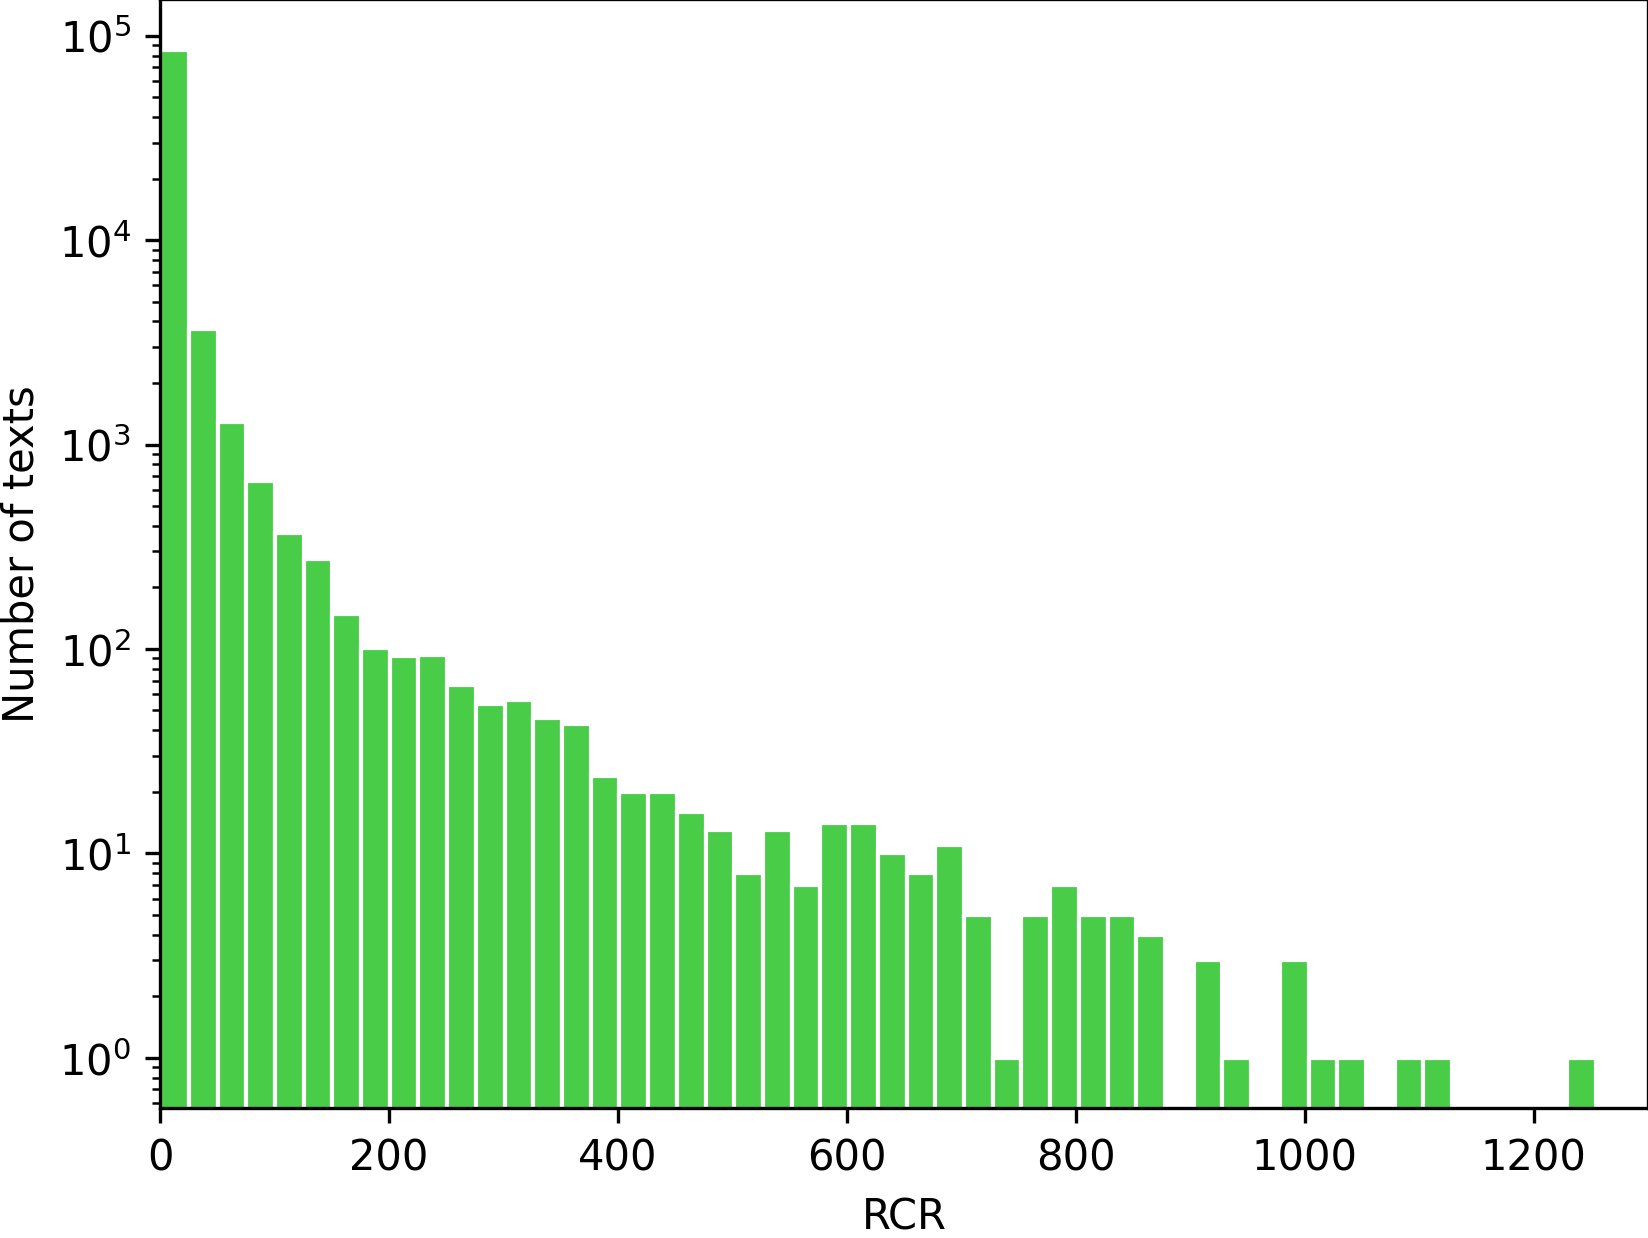
\includegraphics[width=\textwidth]{img/fig_self-compression_histogram.png}
\caption{A histogram representing the self-compression score (RCR) of 96200 Project Gutenberg texts.}
\label{fig:self_compression_histogram}
\end{figure}

Figure \ref{fig:self_compression_histogram} shows how the 92600 texts in this dataset cluster in terms of their RCR. Note that the vertical axis is logarithmic. If the hypothesis that texts with a high RCR are good co-compressors, we should expect some of them to outperform Middlemarch if figure \ref{fig:cocomp_comparison} is re-plotted to include these texts.

This is, almost, what we find in figure \ref{fig:cocomp_comparison_best}. The 30 texts with the highest RCR were selected for inclusion in this plot. As can be seen here, all of these outperform naive LZMA to some degree, with Middlemarch still performing best in the median case. Since this method of measuring RCR works, it may be possible to use it to automatically construct a basis text for a co-compressor that gives a better compression ratio.

\begin{figure}[h!]
\centering
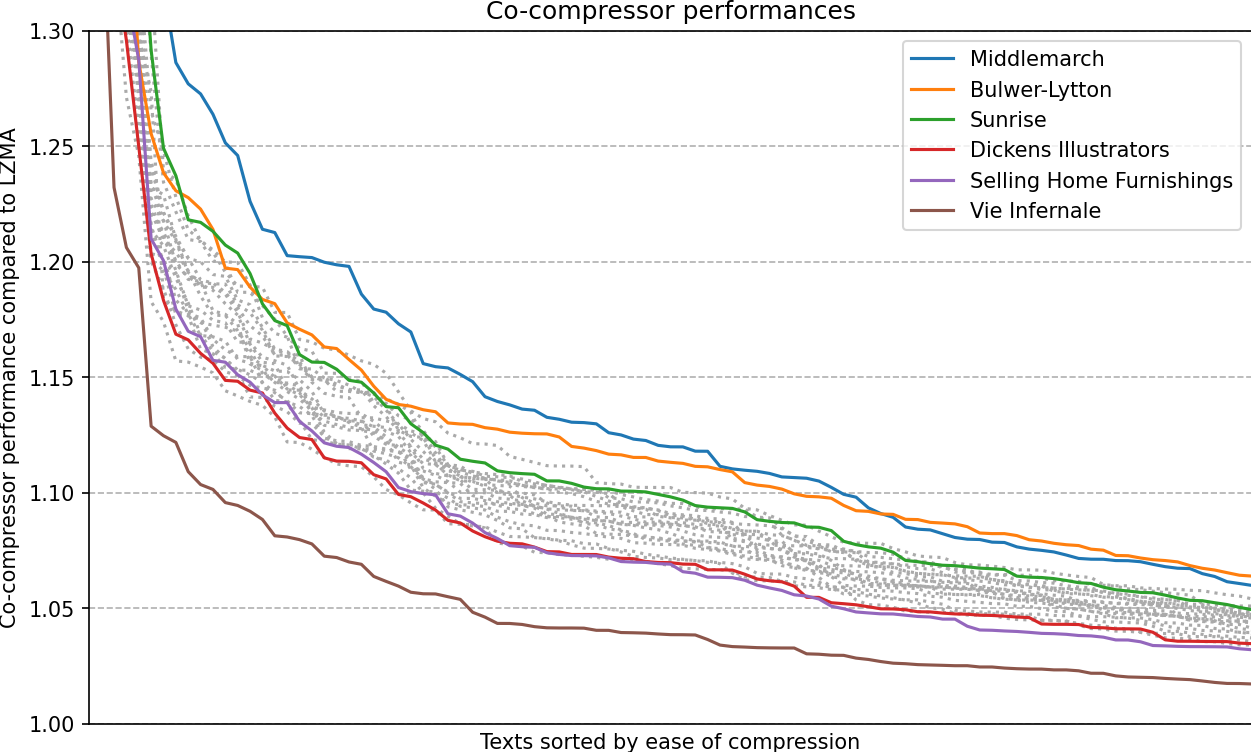
\includegraphics[width=\textwidth]{img/fig_cocomp_performance_best.png}
\caption{The performance of instances of the \texttt{CoCompressor} class trained on 30 texts selected for their high RCR out of a set of 96200 candidate texts. Each line represents a \texttt{CoCompressor}. The value on the vertical axis is the ratio of the size of the encoding produced by naive LZMA to that produced by the \texttt{CoCompressor}, while the horizontal axis goes through possible inputs for comrpession.}
\label{fig:cocomp_comparison_best}
\end{figure}








\subsection{Conclusions and future work}

\todo[inline, color=yellow]{Idea: see if there's a chain of bootstrapping. Middlemarch compresses everything well, but is there something that compresses Middlemarch well? If so, use that as an earlier step in the bootstrapping}
\todo[inline, color=yellow]{Idea: how well does the first half of Middlemarch compress the second half? If the resulting compression is short enough, this facilitates bootstrapping even more: use part 1 to compress part 2, use the total to compress another text. You could also do it in more splits.}
\todo[inline, color=yellow]{Idea: co-compressors take compressors as one of their initializers, but they are themselves compressors. Is there any use in stacking them?}
\todo[inline, color=yellow]{Idea: try to add some noise to a compressed version of something and see if it decompresses into anything}
\todo[inline, color=yellow]{Idea: can you automatically generate a text ex nihilo that will be a good co-compressor using RCR as a metric?}
\todo[inline, color=yellow]{Potential explanation for good co-compressors: file size has sweet spots. There is a repeated pattern of performance getting worse and then suddenly better as file size grows, investigate.}
\todo[inline, color=yellow]{Idea: if the \texttt{CoCompressor} class takes a compression algorithm and improves it, can this method be used recursively on itself (starting with some very naive compression) to get something that performs significantly better?}
\todo[inline, color=yellow]{Why Middlemarch??}
\todo[inline, color=yellow]{Idea for practical compression: start compressed file by indicating what you want to use as a basis text, then give compressed version. Potentially, stack these: if you need basis A to get B and basis B to get C, have the file format allow passing both B and C using basis A.}